\chapter{Grundlagen}
\label{ch:basics}

In diesem Kapitel werden alle notwendigen Fachbegriffe und Abkürzungen eingeführt, die für das Verständnis der fachlichen Einordnung dieser Arbeit erforderlich sind.
Dabei wird auf den Begriff der Aktion im Sportkontext eingegangen, sowie auf verwandte Problemstellungen und auf die historische Entwicklung des Forschungsfeldes, die schließlich zum Deep-Learning führt.

\section{Aktionen und Aktivitäten}
\label{sec:aktionen-und-aktivitaeten}

Um eine \gls{har} zu verstehen, muss zunächst erklärt werden, was eine Aktion ist und welche Art von Ereignissen im Fußball unter diesen Begriff fallen.
Nach Donald Davidson ist eine Aktion durch vier Kriterien gekennzeichnet~\cite{Chen14} (Original nach~\cite{Davidson63}):

\inquotes{There are four aspects to define action in the philosophy of action [...]:
first, action is what an agent can do;
second, action requires an intention;
third, action requires a bodily movement guided by an agent or agents;
and fourth, action leads to side-effects.}

Eine Aktion hat danach folgende Eigenschaften:
\begin{description}
    \item[Ursache] Eine Aktion wird verursacht von einem Spieler und passiert nicht zufällig.
    \item[Absicht] Eine Aktion ist Folge einer höheren Intention.
    \item[Bewegung] Eine Aktion kann nur durch Bewegung eines oder mehrerer Spieler angestoßen werden.
    \item[Nebeneffekte] Eine Aktion verändert seine Umwelt und zieht Konsequenzen mit sich.
\end{description}

In der Literatur wird der Begriff der Aktion häufig in einem ähnlichen Kontext ersetzt durch Aktivität oder Event~\cite{Giancola18}.
Eine Aktivität ist dabei eine Abfolge mehrerer atomarer Aktionen innerhalb eines Zeitfensters~\cite{Dai17}.
Ein Zweikampf kann \zB aus der Abfolge mehrerer Aktionen, wie Dribble und Tackle bestehen.
Damit hält es dennoch der Definition einer Aktion selbst stand.
Vielmehr ist eine Aktivität eine höhere Abstraktion mehrere Aktionen, die sich eher zur taktischen Analyse und weniger zu technischen Analyse eignen.

Ein Event ist hingegen an einen Zeitpunkt gebunden und bezieht sich auf einen bestimmten Kontext, der durch Regeln definiert ist~\cite{Giancola18}.
Ein Beispiel für ein Event ist \ua ein Tor, dessen Entscheidungszeitpunkt klar definiert, in dem der Ball die Torlinie überschreitet.
In Bezug auf die oben genannte Definition kann ein Event als ein mögliches Ergebnis einer Aktion betrachtet werden.
Die Aktion eines erfolgreichen Torschusses führt \zB zu dem Event des Tors.
Alle drei Begriffe haben letztlich gemeinsam, dass sie zeitlich abgrenzbar sind.

In dieser Arbeit wird trotz aller Unterschiede versucht, alle Ereignisse als Aktionen abzubilden.
Das ist zum einen der Natur von neuronalen Netzen geschuldet, die auf ein einheitliches Format angewiesen sind.
Zum anderen lassen sich Events auf Aktionen zurückführen und Aktivitäten in Aktionen zerlegen, sodass eine einheitliche Handhabung möglich ist.
Die Ergebnisse dienen somit primär der technischen Analyse.


\section{Video Understanding}
\label{sec:video-understanding}

Die automatische Videoanalyse (auch Video Understanding) ist einer der schwierigsten Probleme im Bereich Computer Vision und Machine Learning~\cite{Sozykin17,Jiang19}.
Als Video gilt in diesem Zusammenhang eine beliebig lange Sequenz bestehend aus Bildern (\glspl{frame}).
Zur einfacheren Handhabung werden längere Videos meist in kürzere Segmente (\glspl{clip}) mit einer festen Länge von wenigen Sekunden zerlegt.
Während ein (ungeschnittenes) Video viele Aktionen beinhalten kann, sind \glspl{clip} meist so gewählt, dass sich nur eine oder wenige (überschneidende) Aktionen darin ereignen~\cite{Jiang19,Kay17}.
Verschiedene Probleme widmen sich der Analyse von Videomaterial, die teils sehr unterschiedliche Aspekte behandeln:

\begin{description}
    \item[Feature-Extraktion]
    beschreibt die effiziente Komprimierung eines Bilds oder eines kurzen \glspl{clip} auf einen Vektor oder eine Matrix mit fester Größe~\cite{Tran14}.
    Die so gewonnenen Matrizen werden als \gls{feature} oder Feature-Vektoren bezeichnet.
    \item[Feature-Aggregation]
    setzt direkt an der Feature-Extraktion an, indem die komprimierten Features einzelner Frames oder \glspl{clip} zu verschiedenen (meist konsekutiven) Zeitpunkten miteinander verknüpft werden~\cite{Ng15}.
    Die Informationen werden also zeitlich aggregiert.
    \item[Human Action Recognition (HAR)]
    (auch Video Klassifizierung) beschreibt das Erkennen von Aktionen innerhalb eines \glspl{clip}~\cite{Rodriguez08}.
    \item[Action Spotting]
    ist ein spezielles Problem, das auf der \gls{har} aufbaut.
    Ist die Information, dass eine Aktion in einem \gls{clip} stattfindet, bereits gegeben, wird in dieser Aufgabe der genaue Zeitpunkt der Aktion innerhalb dieses \glspl{clip} bestimmt~\cite{Giancola18}.
    Die Aktionen werden also streng genommen als Events behandelt.
    \item[Zeitliche Action Detection]
    beschreibt das zeitversetzte Erkennen von Aktionen in ungeschnittenen Videos.
    Es müssen dabei die Aktionen und die Zeitintervalle, in denen sie sich ereignen, gleichermaßen gefunden werden~\cite{Xia20}.
    \item[Action Detection]
    (auch Action Localisation) erweitert die zeitliche Action Detection zusätzlich um die Bestimmung räumlicher Intervalle (Bounding Box) für jede Aktion~\cite{Xia20}.
    Die Action Detection verhält sich damit analog zur Object Detection, wie die Action Recognition zur Object Recognition.
\end{description}


Die Aufgabenstellung dieser Arbeit entspricht einer \gls{har}, die (perspektivisch) zur Anwendung in eine zeitliche Action Detection eingebettet werden soll.
\autoref{fig:problems} zeigt ein typisches Zusammenspiel der verschiedenen Probleme.
Die Zeitachse entspricht hier den Frames eines Videos.
Dabei werden für eine bestimmte Anzahl an Frames (hier 16) iterativ Features extrahiert.
Der Input für die Feature-Extraktion wird, sofern es sich um mehr als einen Frame handelt, als Chunk bezeichnet.
Diese Chunk-Features werden in einer höheren Instanz zu einem \gls{clip}-Feature (hier aus 64 Frames) aggregiert.
Die Feature-Aggregation ist optional und kann je nachdem, wie viele Frames die Feature-Extraktion verarbeiten kann, entfallen.
In diesem Fall können direkt Features auf \gls{clip}-Ebene generieren werden.
In der Action Recognition lernt das Modell anschließend den Zusammenhang zwischen \gls{clip}-Feature und Label.
Zuletzt kann das \gls{har}-Modell in der zeitlichen Action Detection iterativ benutzt werden, um Intervalle für die Aktionen zu bestimmen.

\begin{figure}[htbp]
    \centering
    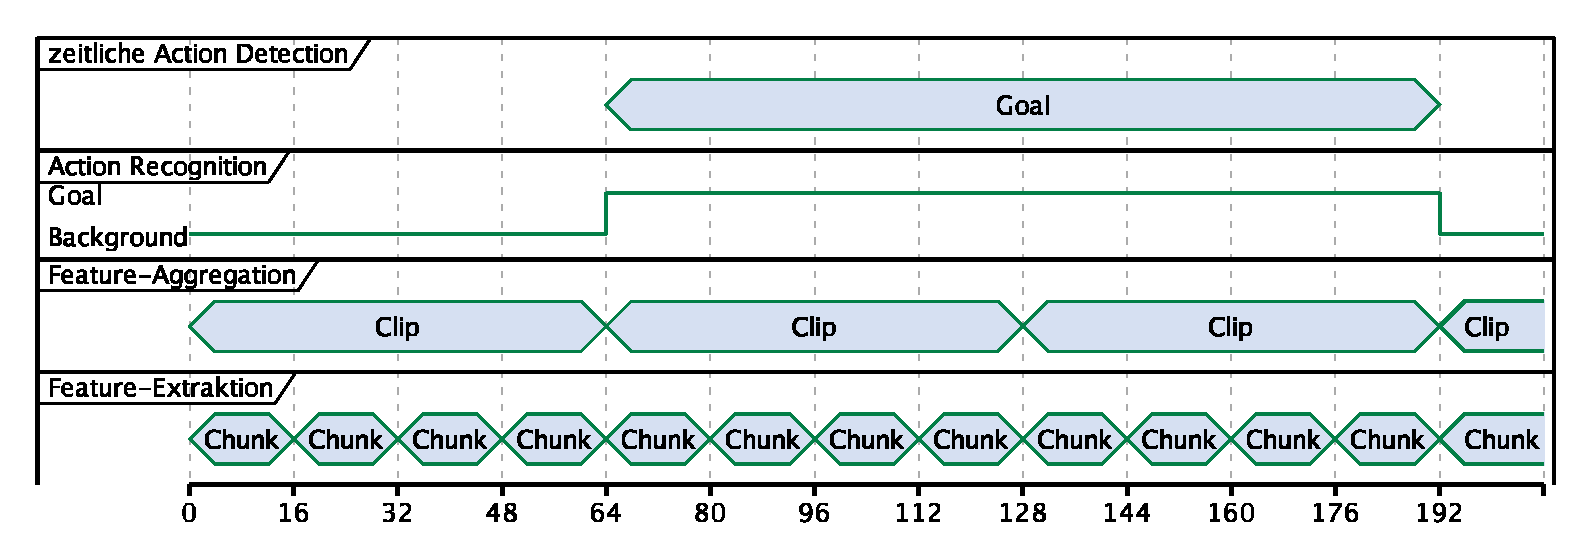
\includegraphics[width=0.9\textwidth, height=0.9\textwidth, keepaspectratio, interpolate]{fig/problems.eps}
    \caption[Teilprobleme im Bereich Video Understanding]{Teilprobleme im Bereich Video Understanding (Quelle: Eigene Darstellung)}
    \label{fig:problems}
\end{figure}

Die Darstellung in \autoref{fig:problems} zeigt eine spezielle (binäre) Form der \gls{har}, die nur zwischen den Zuständen Tor und Nicht-Tor unterscheidet.
Diese binäre Klassifizierung kann zu einer Multi-Class- und zu einer Multi-Label-Variante erweitert werden.
Bei der Multi-Class-Erkennung kann zu jedem Zeitpunkt eine aus $\gls{tld:A}$ Aktionsklassen klassifiziert werden.
Für den Fall, dass sich keine Aktion ereignet, wird ein künstliches Label (oft \emph{Background} genannt) eingeführt.
Im Multi-Label-Fall können sich die Aktionen sogar zeitlich überschneiden, \dh zu jedem Zeitpunkt können $0$ bis $A$ Aktionsklassen erkannt werden.
Die gleichzeitige Erkennung von zwei dicht aufeinanderfolgenden Aktionen innerhalb des gleichen \glspl{clip} ist also nur im Multi-Label-Fall möglich.


\section{Lösungsstrategien}
\label{sec:loesungsstrategien}

Die meisten Ansätze zur Umsetzung einer \gls{har} lassen sich in eine von drei grundlegende Kategorien unterteilen~\cite{Rahmad18, Kothawade19}:

\begin{description}
    \item[Detection \& Tracking]
    Es werden Low-Level-Features erfasst, indem die Akteure (Spieler) in jedem Bild einzeln erfasst und wiedererkannt (getrackt) werden.
    Pro Spieler wird die Differenz zwischen den Bildern (\zB mit Trajektorien oder Optischem Fluss) errechnet, woraus sich ein Bewegungsmuster ergibt.
    Von der Bewegung wird dann auf eine Aktion geschlossen.
    Diese Methode ist allerdings nur bei einer hohen Auflösung einsetzbar und erfordert eine manuelle Anpassung bei abweichenden Daten.
    Ebenso ist die Inferenzzeit vergleichsweise lang.
    Zu den populärsten Methoden gehören \ua \gls{idt}~\cite{Wang13}.
    \item[Feature-Extraktion \& Klassifizierung]
    Bei diesem Ansatz werden Bildinformationen zunächst komprimiert, um die Dimension im Input-Raum zu verkleinern.
    Die \gls{feature}s spezieller Objekte, wie Spielfeldlinien, Spieler oder Spielstandtafel werden einzeln oder als ein globaler Feature-Vektor auf dem Gesamtbild erfasst.
    Bei der anschließenden Klassifizierung werden die Feature-Vektoren mit einem nachgelagertem Klassifizierer (\zB einer \gls{svm}) auf eine Aktionsklasse abgebildet.
    Das Gesamtmodell besteht somit aus mehreren Untermodellen, die jeweils auf verschiedene Aufgaben zugeschnitten sind.
    \item[End-to-end Deep-Learning]
    Diese Ansätze benutzen \glspl{dnn} und bilden alle Zusammenhänge in einem Schritt ab.
    Im Vergleich zu den anderen Ansätzen zeichnet sich Deep-Learning durch seine hohe Zahl von Parametern aus, die optimiert werden müssen.
    Dazu braucht es im gleichen Maße eine hohe Zahl an Beispieldaten.
    Weitere Unterschiede sind eine höhere Rechenlast und damit verbunden eine längere Laufzeit während der Optimierung (\gls{training}).
    Andererseits entfallen bei dieser Methode weite Teile der Vorverarbeitung (Pre-Processing).
    Das Modell erlernt alle Low-Level-Features stattdessen implizit mit~\cite{Rahmad18}.
\end{description}

Vergleicht man die drei genannten Gruppen, so ist nicht nur die Anzahl der Publikationen im Bereich \gls{deep-learning} höher, sondern auch die Genauigkeit der Modelle~\cite{Rahmad18}.
Zudem ist die Umsetzung der beiden übrigen Kategorien aufgrund der aufwendigen Vorverarbeitung wesentlich zeitaufwendiger und würde den Rahmen dieser Arbeit sprengen.
Daher werden im Folgenden ausschließlich \gls{deep-learning}-basierte Ansätze verfolgt.


\section{Neuronale Netze und Deep-Learning}
\label{sec:deep-learning}

\gls{deep-learning}, als Untermenge des Maschinellen Lernens (Machine Learning), setzt auf den Einsatz von Neuronalen Netzen zur Optimierung beliebig komplexer Funktionen.
\glspl{dnn}, die dem menschlichen Gehirn nachempfunden sind, zeichnen sich durch eine Netzwerk-artige Struktur aus, bestehend aus Knoten, die in Schichten angeordnet und miteinander verbunden sind~\cite{Burkov19}.
Das in~\cite{rosenblatt58} erstmals vorgestellte Perceptron (\autoref{fig:dnn} links) ist die einfachste Topologie eines Neuronalen Netzes bestehend aus einem zweischichtigem Netz.
Mit der Hinzunahme weiterer \sog Hidden-Layer zwischen dem Input- und Output-Layer entstehen \emph{tiefe} \glspl{dnn} (auch \gls{mlp}), woher auch der Begriff Deep-Learning stammt~\cite{Burkov19}.
Die in \autoref{fig:dnn} gezeigten grünen Knoten entsprechen sogenannten \fc-Layern (fully-connected), die mit allen Knoten der Vorgänger- und allen Knoten der Nachfolger-Schicht verbunden sind.
Intern können die Layer als Gewichtsmatrizen $W$ repräsentiert werden, die mittels eines Optimierungsverfahren, wie \gls{backpropagation}~\cite{rumelhart86} und anhand von Problem-spezifischer Beispieldaten optimiert werden können.

\begin{figure}
    \centering
    \bigimage{img/02_dnn}{0.4\textwidth}
    \caption{Topologie: \gls{dnn} nach~\cite{Veen17}}
    \label{fig:dnn}
\end{figure}



%Wir betrachten Neuronale Netze als Funktionen $f(x) = y$.
%Das \gls{dnn} erhält einen Input (Reiz) $x$, der über mehrere Schichten entlang der Verbindungen vorwärts propagiert wird und schließlich in einer Senke mündet.
%Jede Schicht wird durch eine Aktivierungsfunktion $\sigma(f_{l_i}) = y_{l_i}$ abgeschlossen, die das Ergebnis in einen bestimmten Wertebereich abbildet.
%Besteht ein Netz aus mehreren Schichten (\gls{layer}) $l_i$, sind diese als Funktionen $f_{l_i}(x) = W_{l_i} * x + b_{l_i}$ definiert, wobei $W$ die jeweilige Gewichtsmatrix und $b$ den Bias-Vektor darstellen.
%Es gilt dann $f(x) = f_{l_L}(\dots(f_{l_2}(f_{l_1}(x))))$ für ein Netz mit $L$ Schichten.
%Ein bestimmter Knoten wird indexiert als $x^{(u_i)}_{l_i}$.
%\autoref{fig:dnn} zeigt zwei mögliche Architekturen topologisch mit zwei \bzw drei Layern.

%\gls{deep-learning} beschreibt den Optimierungsprozess für die Funktion $f$ mit mindestens drei Layern.
%Dabei wird der Fehler für möglichst viele Beispieldaten berechnet und mittels \gls{backpropagation} auf die Gewichte $W_{l_i}$ jedes Layers zurückgeführt.
%So kann der Einfluss jedes Gewichts auf den Fehler bestimmt werden und die Gewichte können einzeln in Proportion zu ihrem Einfluss justiert werden.
%Sofern die Aktivierungsfunktion differenzierbar ist, können alle Parameter innerhalb von $f$ mittels Backpropagation optimiert werden.
%Voraussetzung ist, dass ausreichend viele Beispiele vorhanden sind \cite{Burkov19}.

%Die Aktivierung im letzten Layer ist wiederum abhängig von der Problemstellung \cite{Gugger20}:
%Im Multi-Class-Fall ist die Softmax-Funktion aus \autoref{eq:softmax} weit verbreitet.
%Softmax bildet $y_{i \in \{1, \dots, M\}}$ pro Klasse so ab, dass die Summe Eins ergibt und sich der Classifier für eine der Klassen entscheiden muss.
%Softmax wird in diesem Zusammenhang häufig mit Kreuzentropie (Cross Entropy Loss) als Fehler kombiniert.

%\begin{equation}
%    \label{eq:softmax}
%    softmax(x_i) = \frac{e^{x_i}}{\sum_j e^{x_j}}
%\end{equation}

%Im Multi-Label-Fall funktioniert Softmax nicht, da potenziell mehrere Labelknoten $y_i$ aktiviert werden sollen \cite{Gugger20}.
%In diesem Fall bietet sich, wie auch in der binären Klassifizierung, die Sigmoid-Funktion aus \autoref{eq:sigmoid} an:
%Jeder Knoten wird isoliert betrachtet und der Fehler wird \zB mit binärer Kreuzentropie (Binary Cross Entropy Loss, siehe \autoref{eq:bce}) berechnet:

%\begin{equation}
%    \label{eq:sigmoid}
%    sigmoid(x) = \frac{1}{1 + e^{-x}}
%\end{equation}

%\begin{equation}
%    \label{eq:bce}
%    bce(y, o) = - \sum_{c=1}^A y_{o=c} \log p_{o=c}
%\end{equation}

Abseits von klassischen \glspl{dnn} sind insbesondere die Konzepte von \glspl{cnn} und \glspl{rnn} hervorzuheben.
\glspl{cnn} sind Netze, die häufig im Umgang mit Bildern genutzt werden, da sie besonders gut räumliche Beziehungen abstrahieren können~\cite{Pointer19}.
Hingegen werden \glspl{rnn} für die Verarbeitung sequenzieller Daten und Zeitreihen genutzt~\cite{Pointer19}.
Da Videos sowohl eine räumliche, als auch eine zeitliche Dimension vorweisen, überrascht es nicht, dass Techniken beider Kategorien für die im nachfolgenden Kapitel vorgestellten, aktuellen Lösungsansätze zur \gls{har} relevant sind.
Daher werden die wichtigsten Konzepte und Modelle beider Oberkategorien zum allgemeinen Verständnis der folgenden Kapitel rekapituliert.

\label{sec:conv}

\section{Convolutional Neural Networks}
\label{sec:cnn}

\glspl{cnn} sind Neuronale Netze, die auf die Verarbeitung von Bildern zugeschnitten sind.
Dabei werden lokale (rechteckige) Ausschnitte innerhalb des Bildes mit einem Moving-Window-Ansatz (siehe~\cite{Burkov19}) von links nach rechts und von oben nach unten verarbeitet.
Eine Faltungsmatrix (\gls{kernel}), dessen Werte ebenfalls optimierbare Parameter des Gesamtmodells sind, fährt über das Bild und berechnet pro Pixel das innere Produkt des Kernels mit der umliegenden Nachbarschaft des Pixels.
In einem \conv-Layer (in \autoref{fig:cnn} rosa) werden mehrere Kernel initialisiert, um neue Bilder zu erzeugen.
Das Ergebnis jeder Faltung (Convolution) ist die Ähnlichkeit zwischen dem Kernel und dem Input-Signal.
Stapelt man mehrere \conv-Layer hintereinander, kann man beobachten, dass in den vorderen Schichten Low-Level-Features, wie Ecken, Kanten und farbliche Übergänge gelernt werden, die in tieferen Schichten zu High-Level-Features, wie geometrischen Formen und Mustern kombiniert werden~\cite{Burkov19}.

\begin{figure}[hb!]
    \centering
    \bigimage{img/02_cnn}{0.4\textwidth}
    \caption{Topologie: \gls{cnn} (Quelle:~\cite{Veen17})}
    \label{fig:cnn}
\end{figure}

Pro Layer ergibt sich eine dreidimensionale \gls{feature-map} aus einem Bild pro Kernel.
Die einzelnen Bilder \bzw die Querschnitte einer Feature-Map werden auch als \glspl{channel} bezeichnet.
Der Input des Netzes besteht typischerweise aus drei Kanälen für den jeweiligen \gls{rgb}-Kanal des Farbbilds.
Eine Faltung, wie sie in tieferen Layern vorkommt (mit mehr als einem Kanal als Input), berechnet immer die Summe aller einzelnen Faltungen~\cite{Burkov19}.

Häufig werden \conv- mit sogenannten \pool-Layern kombiniert (\gls{pooling}), die die Bilder pro Kanal auf eine niedrigerdimensionale Version komprimieren.
In diesen Schichten werden die Informationen in den Feature-Maps weiter komprimiert, allerdings ohne zusätzliche Parameter einzuführen.
Einfache Operatoren, wie der Durchschnitt (Average Pooling) oder das Maximum (Max Pooling) werden auf Teilbereiche der Bilder angewandt.
Dabei werden die Kanäle einzeln verarbeitet und nur die räumliche Dimension wird komprimiert.

Yann Lecun stellte 1998 die Grundlagen mit LeNet-5~\cite{Lecun98} vor -- einem \gls{cnn} bestehend aus zwei \conv- und drei \fc-Layern, das Bilder mit $S^2=32 \times 32$ Pixeln klassifizieren kann.
2012 wurde der Ansatz mit AlexNet~\cite{Krizhevsky12} überholt.
AlexNet ist geprägt durch eine tiefere Architektur von 8 Layern, die erstmalige Verwendung der \gls{relu}-Aktivierungsfunktion~\cite{jarrett09} und dem Einsatz von Max- statt Avg-Pooling.
Bilder können hier in einer Auflösung von $S^2=224 \times 224$ verarbeitet werden.
Eine effizientere Weiterentwicklung dessen war VGG-16~\cite{Simonyan15} mit 16 Layern.
Die großen Kernel der vorderen Layer wurden durch die Abfolge mehrerer kleinerer $(3 \times 3)$-Kernel ersetzt, sodass das rezeptive Feld dennoch gleich bleibt.

%\begin{equation}
%    \label{eq:relu}
%    relu(x) = \begin{cases}
%                    0, & \text{if } x < 0\\
%                    x, & \text{else}
%    \end{cases}
%\end{equation}

\subsection{Inception-Blöcke}
\label{subsec:inception-bloecke}

Eine deutlich schlankere Alternative zu VGG-16 wurde 2014 mit InceptionV1 (GoogLeNet)~\cite{Szegedy14} veröffentlicht.
Der Einsatz von sogenannten Inception-Blöcken war der entscheidende Durchbruch.
Inception-Blöcke ersetzen die gewöhnlichen \conv-Layer durch vier parallele Stränge, die am Ende wieder zusammengeführt werden (siehe \autoref{fig:inception}).

\begin{figure}[hb!]
    \centering
    \bigimage{img/02_inception}{0.4\textwidth}
    \caption{Topologie: Inception-Block (Quelle:~\cite{Karim19})}
    \label{fig:inception}
\end{figure}

Jeder Strang beinhaltet eine punktweise Faltung (Pointwise Convolution), wobei mit einem $(1 \times 1)$-Kernel, die Korrelation eines Pixels entlang aller Feature-Maps abbildet und die Anzahl der Feature-Maps dadurch reduziert wird.
Zudem können Filter verschiedener Größe parallel genutzt werden um die Anwesenheit von großen und kleinen Mustern gleichzeitig lokalisieren zu können.
Nach jeder Faltung kommt eine ReLu Aktivierung, die zu einer höheren Nichtlinearität führt~\cite{Pointer19}.

InceptionV1 nutzt unter Ausnahme des Stamm-Blocks (\stem-Layer), ausschließlich Inception-Blöcke, sowie zusätzliche \pool-Layer in insgesamt 22 Schichten.
Durch den Einsatz der Inception-Blöcke fällt der Fußabdruck mit rund 5 Millionen Parametern vergleichsweise klein aus.
Eine Erweiterung des Vorgängers mit deutlich größerem Fußabdruck ist InceptionV3~\cite{Szegedy15}.
Dabei wurden die $(3 \times 3)$-Faltungen durch eine effizientere Kombination asymmetrischer $(1 \times 3)$- und $(3 \times 1)$-Faltungen abgelöst.
Auch die größeren Kernel im \stem-Block werden weiter zerlegt in mehrere $(3 \times 3)$-Faltungen.
In InceptionV4 (2016)~\cite{Szegedy16} wurden noch weitere Inception-Blöcke verwendet, wobei in diesem Modell eine einheitliche Anzahl an Kernels in allen Inception-Blöcken verwendet wird.

\subsection{Residual Learning}
\label{subsec:residual-learning}

Parallel zur Erscheinung von InceptionV1 wurde auch ResNet-50~\cite{He15} und das damit einhergehende Residual Learning vorgestellt.
Residual Learning ist eine Technik zur Vermeidung von Überanpassung (Overfitting) in Neuronalen Netzen.
Overfitting ist die Folge davon, dass das Netz zu viele Freiheitsgrade hat und so Details der vielen Beispieldaten auswendig lernt, anstatt abstrakte Muster darin zu erkennen.
Dieser Effekt war zuvor bei einem nicht ausgewogenen Verhältnis von Tiefe des Netzes zur Anzahl an Trainingsdatensätzen, unvermeidbar~\cite{Gugger20}.

\begin{figure}[hb!]
    \centering
    \bigimage{img/02_identity}{0.5\textwidth}
    \caption{Topologie: \res-Block (Quelle:~\cite{Karim19})}
    \label{fig:residual}
\end{figure}

Beim Residual Learning werden gewöhnliche Knoten eines Layers in \res-Layer integriert.
Dabei wird eine zusätzliche Verbindung (Skip Connection) eingeführt, die den Input und Output des Layers mithilfe einer punktweisen Multiplikation verknüpft (siehe \autoref{fig:residual}).
Optional wird das eigentliche \conv-Layer von zwei punktweisen $(1 \times 1)$-\conv-Layern umgeben, um die Informationen zusätzlich zu verdichten.
Diese Verdichtungen werden auch als Bottlenecks bezeichnet.
\res-Blöcke werden klassisch in vier \res-Layern (\res1 bis \res4) gruppiert.

Sofern die Möglichkeit des Overfittings besteht, ist das Netz nun in der Lage ein Identitätsmapping (Input $\to$ Input) zu lernen, indem es alle Gewichte eines Blocks auf null setzt.
So können überflüssige Blöcke implizit während des Trainings deaktiviert werden und das Netz kann selbst entscheiden wie viele Layer es benötigt.
Zudem wurde in ResNet-50 erstmalig eine Batch Normalisierung~\cite{Ioffe15} genutzt, was wiederum zu einem schnelleren und stabileren Training führt~\cite{Gugger20}.

\subsubsection*{DenseNet}

Eine alternative Weiterentwicklung zu ResNet ist DenseNet (2018)~\cite{Huang18}, welches zusätzliche Verbindungen zwischen Layern, die nicht direkt aufeinander folgen, herstellt.
Dadurch gibt es zusätzliche Verbindungen und Gewichte.
Im Gegenzug braucht es aber eine deutlich geringere Anzahl an Layern und dünneren Feature-Maps.

In einem sogenannten Dense-Block geht der Input aller vorherigen Feature Maps innerhalb des Blocks ein.
So können Features aus früheren Layern wiederverwendet werden und es müssen weniger zusätzliche (und im gewissen Maße redundanten) Features erzeugt werden.
Im Gegensatz zu ResNet werden die eingehenden Features vergangener Layer allerdings nicht mit punktweiser Multiplikation verknüpft, sondern mit \sog Channel-wise Concatenation.
\Dh die Input-Features früherer Layer werden mit den eigentlichen Input-Tensoren konkateniert.
Da die Feature-Maps hierfür jeweils die gleiche Auflösung haben müssen, wird das Netz in mehrere Dense-Blöcke eingeteilt.
Innerhalb der Blöcke wird die Auflösung nicht verändert und alle Layer sind miteinander verbunden.
Zwischen den Dense-Blöcken werden Transition-Layer (\ua mit \pool-Layern) eingebaut, sodass die Auflösung im Hinblick auf die Gesamtarchitektur dennoch reduziert werden kann.

\subsection{Channel-wise Separable Convolution}
\label{subsec:group-conv}

Als letzte Untergruppe seien (Kanal-)separierbare Faltungen (Depthwise \bzw Channel-wise separable convolution) erwähnt.
Mit dem Einsatz in Architekturen, wie Xception (2016)~\cite{Chollet17} oder MobileNet (2017)~\cite{Howard17}, konnte \ua dank weniger Parametern und Rechenoperationen der Einsatz auf mobile Geräten ermöglicht werden.

Separierbare Faltungen bestehen aus einer Faltung pro Kanal und einer Kanal-übergreifenden, punktweisen Faltung.
\Dh jeder Kernel erhält nur Zugriff auf je einen Kanal der vorherigen Feature-Map, sodass die Faltung keine direkte Interaktion zwischen den Kanälen abbildet.
Um dennoch Interaktion abzubilden, folgt auf die Kanal-weise Faltung immer eine punktweise Faltung~\cite{Howard17}.

\section{Recurrent Neural Networks}
\label{subsec:recurrent-neural-networks}

Die zweite Gruppe relevanter Backbone-Modelle stellen \glspl{rnn} dar.
Dazu zählen Neuronale Netze mit einem internen Zustand, mit dem eine zeitliche Abhängigkeit abgebildet werden kann, ähnlich einem Gedächtnis.
Damit sind sie besonders gut geeignet um sequenzielle Daten mit einer zeitlichen Dimension zu klassifizieren.
Topologisch unterscheiden sie sich durch Zyklen innerhalb des Netzwerks (siehe \autoref{fig:rnn}).

\begin{figure}[h!]
    \centering
    \bigimage{img/02_rnn}{0.2\textwidth}
    \caption{Topologie: \gls{rnn} (Quelle:~\cite{Veen17})}
    \label{fig:rnn}
\end{figure}

In seiner Reinform speichert ein \gls{rnn} zu jedem Zeitpunkt $t_i$ für den Input $x_{t_i}$ zusätzlich ein Hidden State $h_{t_i}$, der als zusätzlicher Input im nächsten Zeitpunkt $t_{i+1}$ genutzt wird.
Jeder Block hat also eine Rückkopplung zu seinem vorherigen Zustand.
Diese Architektur leidet allerdings besonders am \gls{vanish-gradient}.
Ab einer gewissen Tiefe wird der Einfluss des Fehlers, welcher während der Backpropagation ermittelt wird, verschwindend (vanishingly) gering und das Netz kann im schlimmsten Fall nicht weiter optimiert werden~\cite{Pointer19}.

\subsection*{Long Short-Term Memory (LSTM)}

In der ursprünglichen Form ist es schwer längere zeitliche Zusammenhänge zu erkennen.
Die LSTM-Architektur~\cite{Hochreiter97} erweitert die gewöhnliche \gls{rnn}-Architektur dadurch, dass es die eine explizite Funktion hat, Gelerntes wieder zu vergessen.
Wie viel vergessen wird, ist somit Teil des Trainings, womit es ein längeres Kurzzeitgedächtnis hat als ein reines \gls{rnn}.
Das wird möglich durch den Einsatz verschiedener sogenannter Gates:
Das Input-Gate entscheidet darüber, wie stark der Hidden state (aus dem vorherigen Zeitschritt) in Abhängigkeit von neuem Input geändert wird und der Forget-Gate entscheidet, wie viel alte Information vergessen wird.
Zuletzt entscheidet der Output-Gate darüber welche Informationen an das nächste Layer weitergegeben werden~\cite{goodfellow16, Pointer19}.

\subsection*{Gated Recurrent Units (GRU)}

GRUs~\cite{Cho14} sind eine alternative, schlankere Variante zu LSTMs, wobei Output- und Forget-Gate in eine Einheit (Reset-Gate) überführt werden.
Somit gibt es weniger Parameter und Rechenoperationen.
Auch wenn diese Generation vom RNNs deutlich jünger ist, lässt sich nicht abschließend beurteilen, welche Gruppe die besseren Ergebnisse liefert~\cite{Pointer19}.

